\chapter{Methodology}

\section{Salinity Measurement Method}
A \gls{ctd} sensor, which measures salinity using conductivity, temperature and depth, was chosen as the salinity measurement device.
When choosing a measurement technique multiple factors needed to be considered.
Firstly, the salinity measurements are to be conducted in the Antarctic, where the environment, and remote nature of the area, make majority of the measurement methods unusable.
Secondly, the device would need to fit through an ice core hole with a diameter of $100mm$, and lastly, the device would need to be able to take continuous measurements.

\gls{ctd} sensors do not require sample collection, unlike chlorinity titration, gravimetric analysis and refractometry.
This removes both the need for sample collection and the challenges of sample degradation, storage and transport logistics.

Modern \gls{ctd} sensors are compact, and can easily be designed for specific space constraints.
This coupled with its deployments flexibility make it the preferred choice over methods, such as laboratory methods, which suffer from deployment constraints.
\gls{ctd} sensors allow for continuous realtime monitoring, a characteristic none of the the alternative methods provide.
The alternative methods either require sample collection, or cannot measure continuously.

\gls{ctd} instruments inherently measure conductivity, temperature and pressure simultaneously, providing salinity measurements with temperature and depth compensation, whereas laboratory methods measure salinity only, and require seperate temperature measurements.


These factors coupled with the researcher's significant experience with PCB design and electronics influenced the choice for a \gls{ctd} sensor.

\section{Electrode Design}
When measuring conductivity, choosing an electrode material plays a significant role in the accuracy of the measurements.
To get an accurate measurement of the resistance of the water, ideally, a electrode resistance of zero is required.
This would allow the resistance measurement to be entirely due to the resistance of the water.
Most conductive materials have conductivities of order $10^6 - 10^8 S/m$, which is negligible compared to sea (salt) water, which has an average conductivity of $3.31 S/m$~\cite{conductivities}\cite{ocean_conductivity_tyler}.
Preferably, the material with the highest conductivity, silver, would be used. However, conductivity is not the only factor considred when designing an electrode. 
The electrodes will be submerged in saltwater, which is highly corrosive. The material chosen will require high corrosive resistance. 
Silver, though having the highest conductivity, has a low corrosion resistance, and therefore cannot be used in this application~\cite{zhang_silver}.

Titanium is the material of choice for ocean-use~\cite{materials_ocean_structures}. It is essentially corrosion-free, and offers a conductivity of $2.68\times 10^{6}$~\cite{conductivities}.
However, titanium is expensive and fell out of the budget of this project.
Gold boasts both a high conductivity of $4.10\times 10^{7}$, higher than titanium but lower than silver, and a high corrosion resistance, making it an ideal choice.
Gold is also a commonly used material in electronic design, with it being used in \gls{pcb} manufacturing, to protect copper pads from corrosion.
This is done through a \gls{enig} plating process, where a layer of nickel is chemically deposited onto the exposed copper traces, to prevent the copper from oxidizing, and then a layer of gold is applied over the nickel through an emmersion process, to protect the nickel.
This process is significantly more expensive compared to standard \gls{pcb} manufacturing, however, it allowed for the use of gold electrodes, and therefore was factored into the budget. 

In order to utilise the \gls{enig} process a \gls{pcb} was used to design the gold electrodes.
This allowed the electrodes to be designed with a known area and seperation distance, allowing for accurate conductivity calculations.
A solder pad was used to design the portion of the \gls{pcb} that would act as the electrode, since it allowed the copper/gold to be exposed.
Then during manufacturing \gls{enig} was chosen as the surface finish, to achieve the gold finish.

The \gls{pcb} was designed to allow for easy calculation of the conductivity $\sigma$, using the equation below:
\begin{equation}\label{eqn:conductivity}
    \sigma = \frac{L}{RA}
\end{equation}

where $L$ is the distance between the electrodes, $R$ is the resistance of the water, and A is the cross-sectional area of the electrodes.
A square face of $20mm\times 20mm$ was chsoen to allow for easy cross-sectional area calculations, and a distance of $10mm$ was chosen as the seperation distance.
This distance was chosen as it is close enough to reduce current spreading, but not too small to where the water could not flow easily between the electrodes.
A $2mm$ fringe guard was added around the main electrode area to reduce current fringing, which is an effect that causes the current to spread beyond the edges of the gap~\cite{roshen_fringing}.
The fringe guards counteract this by saturating the area surrounding the main pads with current, preventing them from fringing.

The resistance of the electrodes was calculated using the Equation~\ref{eqn:conductivity} and was found to have an approximate resistance of $7.55\Omega$

The electrode \gls{pcb} was designed with the consideration of mounting to the probe \gls{pcb}.
To accomodate this, solder pads were added to allow the electrodes to be soldered to the probe \gls{pcb}.
Supports were also factored into the design to ensure that the electrodes stayed straight and secure.
The design can be seen in Figure [insert figure].

\section{Resistance Measurement}
There are multiple ways to measure resistance, however most rely on the same principle, which is the voltage divider principle.
This principle works by using a series circuit with two resistors, and a constant known input voltage.
The voltage over each of the resistors will be proportional to their resistance, and therefore, if the resistance of one resistor is known, the resistance of the other can be calculated.
A simple voltage divider circuit can be seen in Figure~\ref{fig:voltage_divider}.

\begin{figure}[H]\label{fig:voltage_divider}
    \centering
    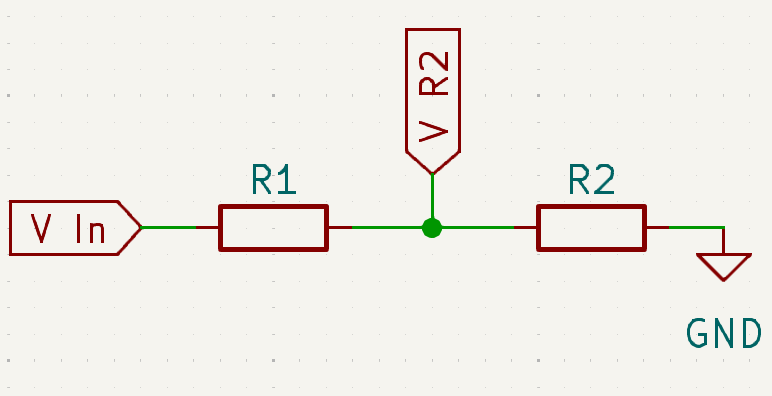
\includegraphics[width=0.6\textwidth]{figures/fig_voltage_divider.png}
    \caption{Simple voltage divider circuit used for resistance measurement.}
\end{figure}

Equations \ref{eqn:voltage_divider} and \ref{eqn:resistance_divider} are used to calculate the resistance from the voltage divider equation.
\begin{equation}\label{eqn:voltage_divider}
    V_{R2} = V_{In} \times \frac{R_2}{R_1 + R_2}
\end{equation}
\begin{equation}\label{eqn:resistance_divider}
    R_2 = \frac{R_1 \times V_{R2}}{V_{In}-V_{R2}}
\end{equation}


\section{Circuit Design}
\subsection{Probe Circuit}
The probe circuit is the circuit which contains the resistor divider, was designed to be printed onto a \gls{pcb}.
This design was influenced by Reference \cite{cam_clark}, where a similar device was designed.





For this application the electrodes were chosen as the R2 resistor, with R1 being a large resistor of known resistance.
Three alernative values of R1 were chosen, to accomodate for any circuit errors.
These values were chosen to be $100\Omega$, $1K\Omega$ and $10K\Omega$.
These values would be used when the resistance between the probes was $1-10\Omega$, $10-100\Omega$, and $100-1K\Omega$ respectively.

Since the electrodes had an expected resistance of $7.55\Omega$, falling into the $1-10\Omega$ range, this would allow for a minumum resolution of $11\%$ of $V_{DAC}$ and maximum of $100\%$ of $V_{DAC}$, for the voltage measurement by the \gls{adc}, as shown in Equations~\ref{eqn:dac_11} and~\ref{eqn:dac_100}.
\begin{equation}\label{eqn:dac_11}
    \frac{1\Omega}{1\Omega + 100\Omega}\times V_{DAC} \times 11 = 11\% V_{DAC}
\end{equation}

\begin{equation}\label{eqn:dac_100}
    \frac{10\Omega}{10\Omega + 100\Omega}\times V_{DAC} \times 11 = 100\% V_{DAC}
\end{equation}
